\documentclass[12pt]{article}
\usepackage{graphicx}

\begin{document}

\setcounter{figure}{0}
\makeatletter
\renewcommand{\thefigure}{S\@arabic\c@figure}
\begin{figure}
%\center{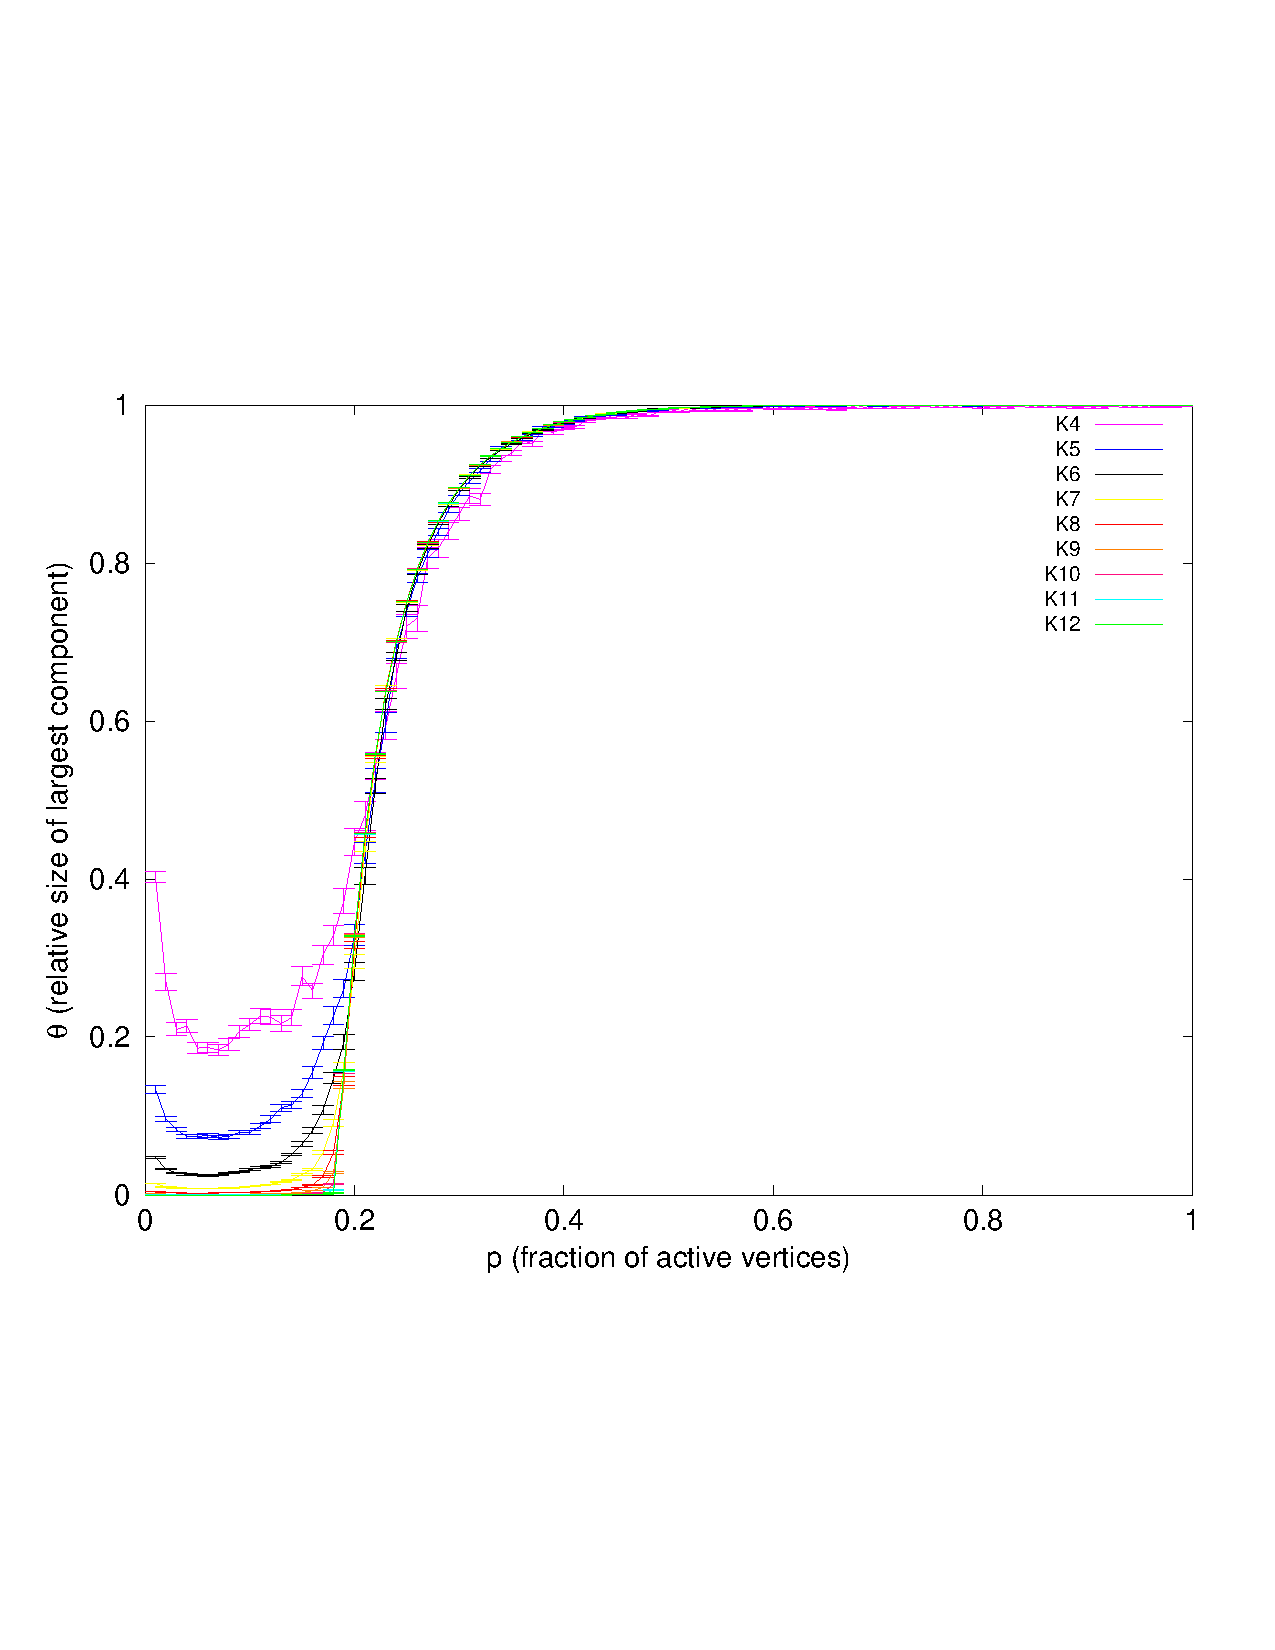
\includegraphics[width=5in]{s1}}

\caption{Demonstration of k independence by determining the
  percolation threshold with multiple values of k (5-12).  $p$ on the
  x axis is the fraction of nodes present, and $\theta$ on the y axis
  is the fraction of nodes in the largest component.  Lower values of
  k have greater finite size sampling errors.}

\label{fig:kindependence}
\end{figure}

\clearpage

\begin{figure}
%\center{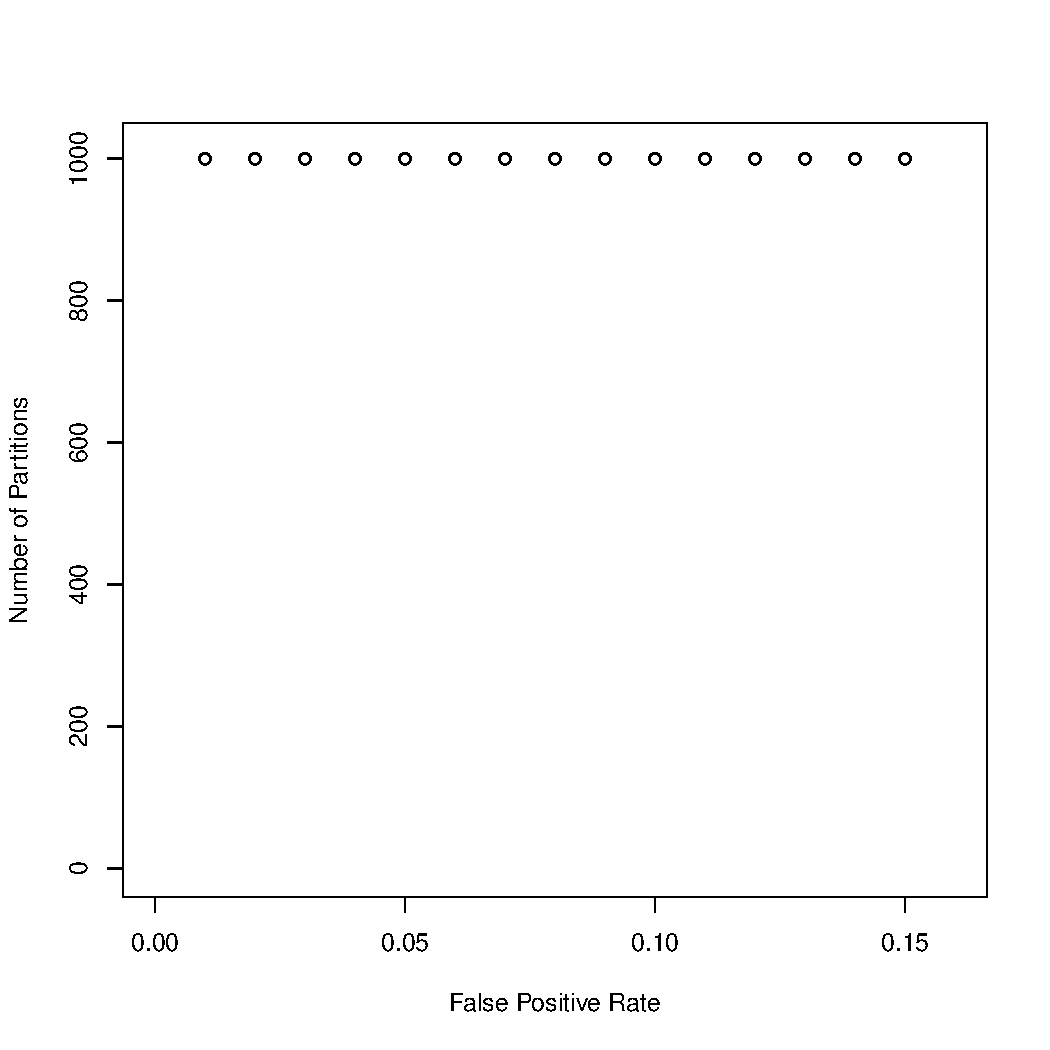
\includegraphics[width=5in]{newpart}}

\caption{The graph shows the number of partitions for a simulated dataset with
  1,000 contigs of 10,000 bp each (circles). For $n=5$ different
  combinations of hash table sizes, there was no variation in results
  for the simulated dataset.}

\label{fig:partfp}
\end{figure}

\end{document}
